\begin{figure}[ht]
\centering
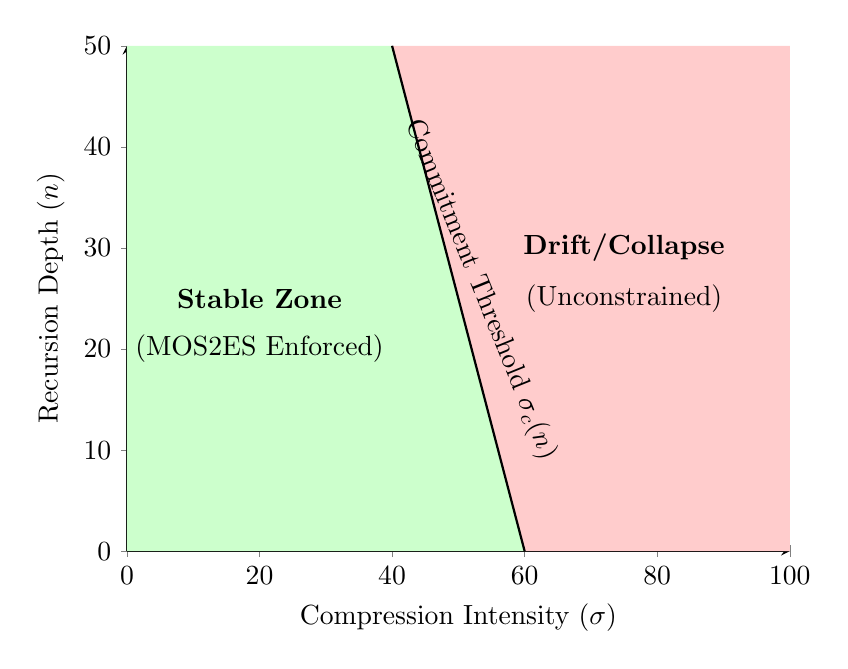
\begin{tikzpicture}
\begin{axis}[
    width=10cm, height=8cm,
    xlabel={Compression Intensity ($\sigma$)},
    ylabel={Recursion Depth ($n$)},
    xmin=0, xmax=100,
    ymin=0, ymax=50,
    axis lines=left,
    view={0}{90}
]

% Define the Stable Zone (Green)
\fill[green!20] (axis cs:0,0) -- (axis cs:60,0) -- (axis cs:40,50) -- (axis cs:0,50) -- cycle;
\node at (axis cs:20,25) {\textbf{Stable Zone}};
\node at (axis cs:20,20) {(MOS2ES Enforced)};

% Define the Collapse Zone (Red)
\fill[red!20] (axis cs:60,0) -- (axis cs:100,0) -- (axis cs:100,50) -- (axis cs:40,50) -- cycle;
\node at (axis cs:75,30) {\textbf{Drift/Collapse}};
\node at (axis cs:75,25) {(Unconstrained)};

% The Boundary Line
\draw[thick, black] (axis cs:60,0) -- (axis cs:40,50);
\node[rotate=-68, anchor=south] at (axis cs:50,25) {Commitment Threshold $\sigma_c(n)$};

\end{axis}
\end{tikzpicture}
\caption{Two-dimensional stress regime map showing compression intensity versus recursion depth. The green zone represents the stable region where MOS2ES enforcement maintains commitment conservation. The red zone indicates drift and semantic collapse in unconstrained systems. The boundary line defines the critical threshold $\sigma_c(n)$ as a function of recursion depth.}
\label{fig:stress-regimes}
\end{figure}
